% 第一章 绪论
\chapter{绪论}
\section{研究背景}
\subsection{智能驾驶测试对海量长尾场景的需求矛盾}
随着智能驾驶技术快速发展起来,它的测试需求也变得日益复杂且多样化,智能驾驶系统需要在各类复杂多变交通场景下\cite{abeysirigoonawardena2019adversarial},展现出可靠性能来确保驾驶安全与舒适,然而现实交通环境里存在海量长尾场景,这些场景虽出现频率低但发生时会对系统构成严峻挑战。

长尾场景的复杂性主要体现在如下几个方面,首先交通环境动态性极强,车辆\ref{fig:vehicle_sample}、行人以及非机动车等交通参与者行为模式千变万化,比如在城市道路当中行人可能突然横穿马路,非机动车可能随意变道或者逆行,\cite{bagschik2018ontology}这些行为都可能引发潜在的碰撞风险,智能驾驶系统必须能够准确感知并预测这些行为,然后做出合理决策。其次道路条件的多样性增加了测试场景的复杂性\cite{biggio2013evasion},从城市快速路到乡村小道,再从高速公路到山区道路,不同道路几何形状、路面状况、交通标志和信号灯等都不一样,智能驾驶系统需要在这些不同道路条件下都能正常运行\cite{brown2020language}。此外天气条件和光照条件的变化,也会对智能驾驶系统的感知和决策造成影响,雨、雪、雾等恶劣天气会降低传感器的性能,不同光照条件像强光、弱光、逆光等会影响视觉系统识别效果。

为了保证智能驾驶系统具备安全性和可靠性,测试过程得覆盖尽可能多的长尾场景,然而这面临着巨大挑战,一方面长尾场景数量庞大几乎无法穷尽,要完全覆盖所有可能场景几乎是不可能任务,另一方面这些场景出现频率较低难以在实际道路测试中频繁遇到,所以传统测试方法往往难以满足智能驾驶系统对海量长尾场景的测试需求,使得测试的充分性和有效性受到限制\cite{cai2020summit}。
\begin{figure}[h]
	\centering
	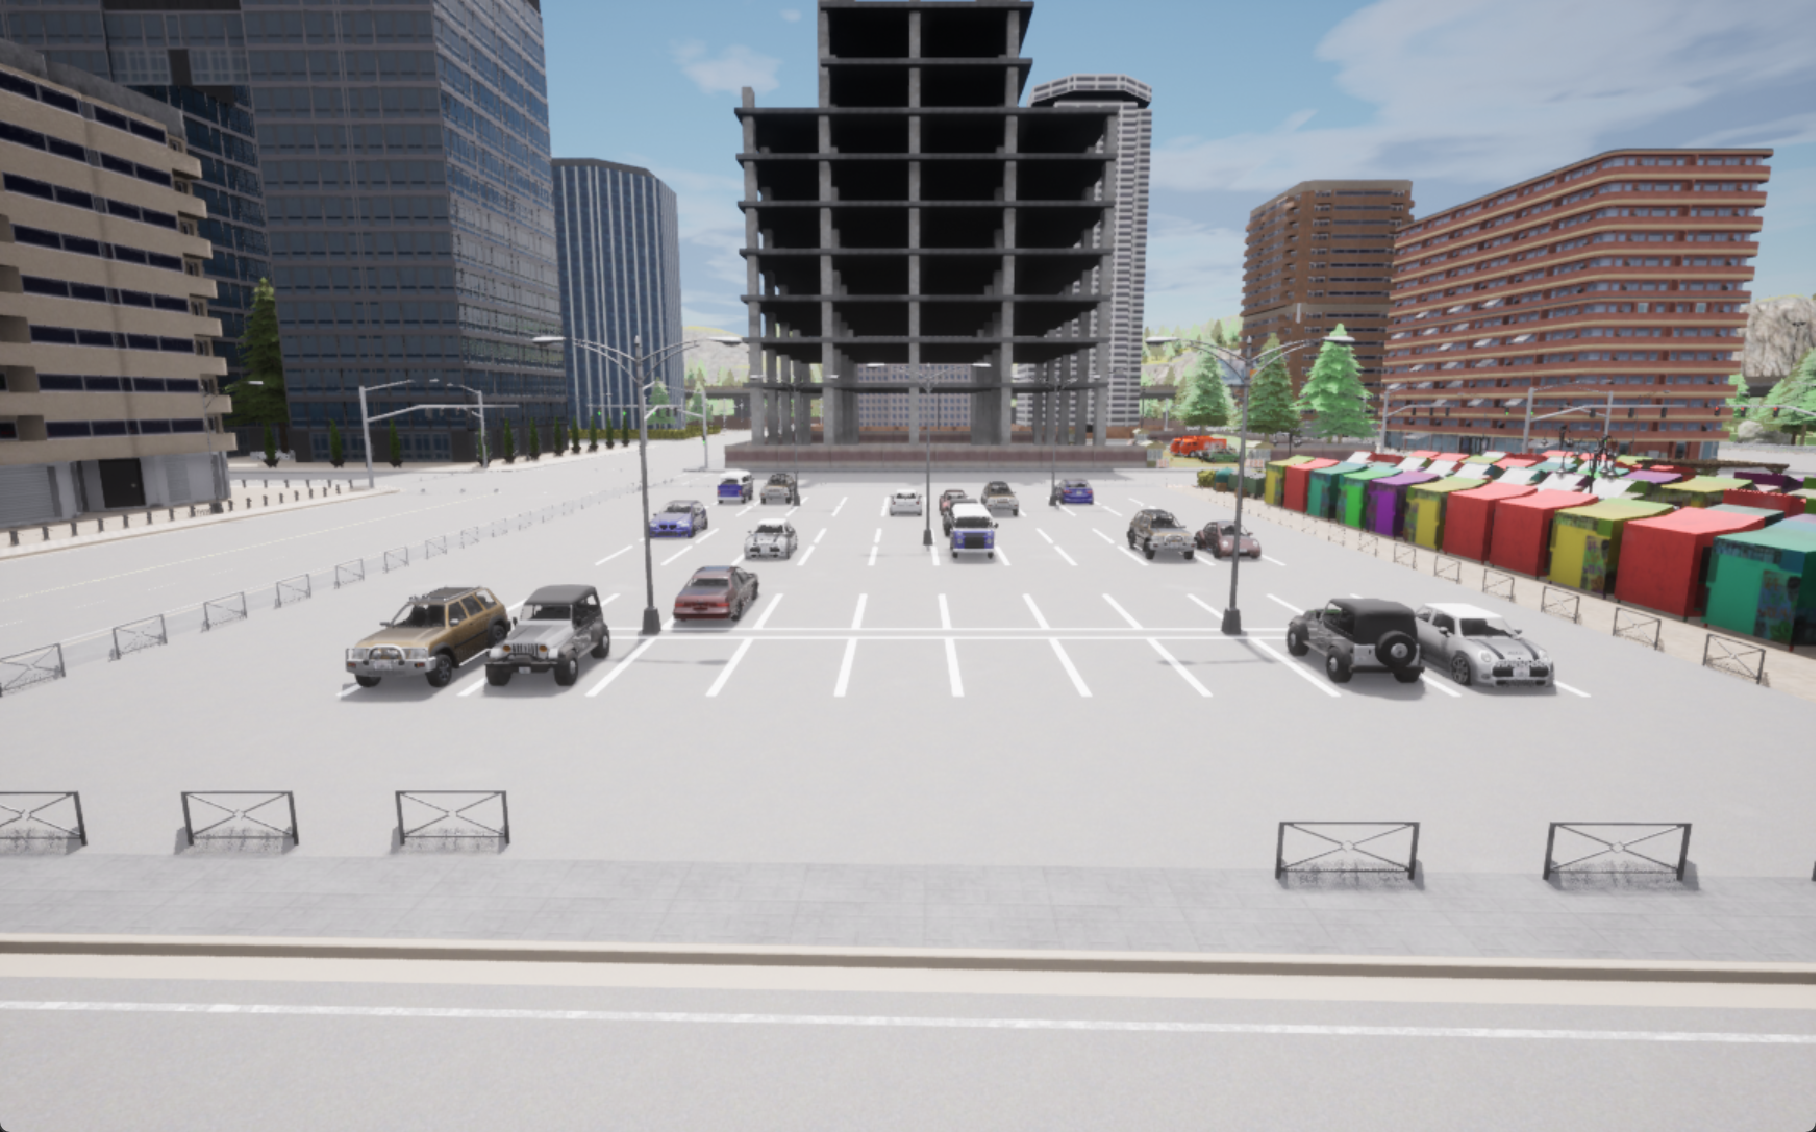
\includegraphics[width=1.0\textwidth]{"images/车辆样式图.pdf"}
	\caption{车辆样图}
	\label{fig:vehicle_sample}
\end{figure}
\subsection{传统场景构建方法的人力成本与效率瓶颈}
在智能驾驶测试这个领域当中,传统的场景构建方法主要靠人工设计和开发\cite{cui2023chatlaw},这些方法虽说在一定程度上能够满足测试需求,不过也存在着比较显著的局限性,人工设计场景需要投入大量专业人员,这些人员要具备交通工程、计算机科学和智能驾驶技术等多学科深厚知识,能准确理解并模拟各种复杂交通场景,这样的专业人才相对比较稀缺,培养成本也十分高昂,随着测试需求不断增加,对专业人员的需求也持续增长,这进一步加剧了人力成本方面的压力。

其次人工设计场景的效率相对比较低,设计一个复杂交通场景需经多步骤,像需求分析、场景建模、代码编写和调试等,每一个步骤都要耗费大量时间精力,例如在场景建模阶段要精确去定义道路几何形状、交通参与者初始位置和行为模式等,在代码编写阶段需把这些模型转化成可执行代码,这不仅要求具备专业编程技能,还需反复调试来确保代码正确性和稳定性,所以人工设计场景速度远不能满足智能驾驶系统快速迭代和测试的需求,此外人工设计场景的准确性和一致性难保证,因为不同设计人员理解和经验存在差异,可能致使设计出的场景出现一定的差异,并且在复杂场景中人工设计易遗漏关键细节,进而影响测试结果准确性和可靠性。

\subsection{大语言模型在代码生成领域的突破性进展}
近年来大语言模型在自然语言处理领域取得巨大突破且逐渐拓展到代码生成等领域,大语言模型通过在海量文本数据上预训练学习到语言语法语义和逻辑结构能生成自然流畅且符合逻辑的文本内容,这种能力为解决智能驾驶测试场景构建难题提供新的思路。在代码生成领域大语言模型已经展现出强大能力\cite{chowdhery2022palm},通过对代码数据学习大语言模型能理解代码结构和逻辑生成符合语法规范的代码片段,例如一些基于大语言模型的代码生成工具可根据用户输入自然语言描述自动生成相应代码实现,这些工具在软件开发领域得到广泛应用显著提高代码开发效率和质量。大语言模型在代码生成中的优势主要体现在以下几个方面:

首先它能够快速生成代码大大缩短开发周期,传统人工编写代码需经过需求分析设计编码和调试等多个阶段且每个阶段都耗费大量时间,而大语言模型可根据输入描述直接生成代码减少中间环节提高开发效率\cite{feng2021intelligent},其次大语言模型生成的代码质量较高,它能学习到代码最佳实践和规范生成的代码不仅符合语法规范还具有良好可读性和可维护性,

此外大语言模型还能根据不同需求生成多样化代码实现为开发者提供更多选择。把大语言模型运用到智能驾驶测试场景构建当中\cite{kong2020physgan},能够充分发挥它在代码生成领域的优势来解决传统方法面临的困境,借助将自然语言描述的测试场景需求转变为代码实现,大语言模型能够快速生成高保真的测试场景进而提高场景构建的效率和质量,结合智能驾驶领域的专业知识还可以进一步优化大语言模型的性能让它更好适应智能驾驶测试场景构建的需求。



	
\section{国内外研究现状}
\subsection{基于大语言模型能够根据人的自然语言指令生成Scenic场景代码}
随着大语言模型像GPT -3、T5等的广泛应用起来,基于自然语言描述生成仿真场景代码成为自动驾驶仿真研究重要方向,自然语言描述能够以简单且直观的方式传递场景信息\cite{klischat2020scenario},传统手工编写场景代码的方式存在效率低且灵活性差的问题,所以如何利用自然语言生成交通仿真场景脚本成为该领域核心问题。
	
大语言模型像GPT - 3和T5这类\cite{Xu2023DriveGPT4},已经成功应用于自然语言到场景代码的转换工作,经过训练之后,这些模型能够理解复杂的自然语言输入内容,依据相关描述,它们可以生成结构化的Scenic脚本文件\cite{scenario_runner_contributors2019carla},这些模型通过解析用户给出的自然语言指令,来生成符合自动驾驶仿真要求的场景代码,比如,\cite{Chen et al. (2022)}提出一种基于GPT的框架,能根据自然语言描述生成含车辆行人交通灯等元素的完整交通场景配置。
	
挑战与进展方面大语言模型生成场景代码有一定进展但仍面临挑战,首先处理自然语言中歧义和模糊性是个难题,复杂场景描述下生成场景可能无法完全符合预期,其次现有模型生成能力处理复杂或特殊交通场景时存在局限性,所以增强语言模型语义理解和场景生成准确性仍是活跃研究领域
	
	\subsection{将场景代码合成合理的智能驾驶场景}
把生成的Scenic场景代码转化成合理的智能驾驶仿真场景,这是实现自动驾驶测试与验证的关键步骤,生成的场景不仅要符合交通方面的规则,还得能够模拟真实的驾驶环境来进行有效测试。
	场景代码转化到仿真环境方面,当前的研究重点主要集中在怎样把大语言模型所生成的Scenic脚本转化成仿真平台能够执行的场景配置内容。例如,\cite{Xie et al. (2021)}开发出基于Scenic的编译器用于把自然语言生成场景描述转化为CARLA仿真平台所需配置文件,通过这种方式生成的场景能够在高保真的仿真环境里进行验证
	
智能场景合成跟动态行为建模这方面,智能驾驶场景不只是包含像道路、交通标志这类静态元素,还涵盖如车辆行驶、变道、停车等动态行为,研究者们提出了多种动态行为建模的方法,让生成的交通场景能更真实地反映驾驶行为与交通流情况,例如,\cite{Zhao et al. (2020)}提出一种基于行为模型的动态场景合成方法来通过模拟交通参与者行为生成交互式智能驾驶环境。
	
复杂交通场景面临的挑战是,虽说场景合成方法在持续发展,但生成复杂真实且符合交通规则的场景依旧是技术难题,现有的场景生成方法在应对复杂交通场景时,可能会出现车辆行为不自然以及交通规则不严谨等状况,所以提高场景合成的灵活性和复杂性仍是研究重点。
	
	\subsection{对生成的交通场景进行展示和效果的量化衡量}
	在生成交通场景之后对其进行展示以及量化评估是保证场景质量和仿真结果准确性的关键步骤,通过对场景开展可视化以及量化评估研究人员能够验证场景的有效性并为后续自动驾驶算法优化提供数据支撑。
	
	可视化展示就是把生成的交通场景借助可视化工具进行展示,从而方便进行人工验证和审阅。\cite{Dai et al. (2020)}我这边提出一种基于关键帧截取的可视化方法,通过在仿真过程当中截取关键帧图像,以此帮助研究人员快速了解仿真过程里的交通场景,结合深度学习相关技术,自动驾驶系统还可以从这些图像当中提取重要信息,进而对场景开展进一步分析与优化。
	
提出量化评估指标的情况是,为了能系统地对生成场景的质量进行评估,许多研究都提出了量化评估框架。例如,\cite{Dai et al.(2020)}提出一种涵盖场景语义保真度等多方面的多维度评估方法,这些评估指标既能反映生成场景的真实性又能助研究人员评估仿真结果有效性。
	
	安全性与性能评估:自动驾驶系统在仿真环境中的表现也需要量化评估。\cite{Li et al. (2021)}提出一种基于自动驾驶系统安全性的评估框架,通过对车辆在生成场景里碰撞率与通过率等指标进行分析,以此评估自动驾驶系统于不同场景之下的安全性和稳定性,借助这样的量化评估手段,研究人员可识别出潜在的风险和问题并进一步优化自动驾驶算法。
	
	\section{研究内容}
	\subsection{面向场景描述的领域知识图谱构建}
在自动驾驶测试场景生成这个事情当中,构建面向场景描述的领域知识图谱是实现高效且准确场景生成的基础,领域知识图谱通过整合自动驾驶领域的专业知识\cite{Wang2021advSim},像交通规则、道路类型、车辆行为模式以及传感器特性等内容,为自然语言描述的解析和形式化代码的生成提供丰富上下文信息和语义支持。
	
领域知识图谱构建包含多个关键步骤\cite{Xu2022Safebench},首先要对自动驾驶领域知识做系统梳理与分类,明确知识的层次结构和关联关系,这涵盖对交通场景里实体(像车辆、行人、道路、交通标志等)及其属性(例如位置、速度、类型等)的定义,还有这些实体之间关系(比如车辆与道路的交互、车辆与行人的避让等),构建知识图谱可将这些复杂知识结构化表示出来,方便后续进行查询和推理。
	
在知识图谱的构建过程当中需要考虑知识动态更新与扩展\cite{Yang2020SurfelGAN},自动驾驶技术处于不断发展中新交通规则车辆类型等不断涌现,所以知识图谱得具备良好可扩展性以及可更新性,通过持续开展知识更新能确保知识图谱始终保持最新状态,进而为场景生成提供准确无误的知识方面支持。
	
除此之外领域知识图谱的构建还得考虑知识表达与存储方式,知识图谱一般是以图的形式进行存储的\cite{Yao2022React},其中节点所表示的是实体而边表示实体间的关系,这种结构化的存储方式不仅方便知识的查询和推理,还能够支持复杂的知识融合与关联分析,借助知识图谱的构建能够实现对自动驾驶场景描述的深度理解和语义解析,为后续的代码生成以及场景合成提供坚实可靠的基础。
	
	\subsection{基于LLM的语义约束代码生成方法}
基于大型语言模型(LLM)的语义约束代码生成方法是达成自动驾驶测试场景高效生成的一项关键技术,大型语言模型(LLM)具备强大的语言理解和生成能力可依据自然语言描述生成高质量形式化代码,不过为保证生成代码的准确性与可靠性需在代码生成过程中引入语义约束机制\cite{Zhang2023CAT}。
	
语义约束代码生成方法的关键是把自然语言描述的语义信息转成代码生成约束条件,这些约束条件涵盖交通规则、道路类型以及车辆行为模式等内容,目的是保证生成的代码既符合语法规范又能满足实际场景语义要求\cite{Zhang2022AdversarialRobustness},借助语义约束机制可有效避免生成代码里的逻辑错误与不符合实际场景的状况,以此提高代码的质量和可用性。
	
实现语义约束代码生成的时候要充分利用LLM语言理解与生成能力\\ \cite{Zheng2023JudgingLLM},LLM可通过对自然语言描述深度理解提取关键语义信息,再将这些关键语义信息转化为代码生成约束条件,同时还得开发对应算法和工具把约束条件嵌入代码生成过程,以此确保生成代码能准确反映自然语言描述语义内容,此外语义约束代码生成方法也需考虑代码可读性和可维护性,生成代码不仅要符合语法和语义规范,还得具备良好结构和注释以方便后续修改和扩展,借助基于LLM的语义约束代码生成方法能实现从自然语言描述到形式化代码高效转换\cite{zhong2023language},可为自动驾驶测试场景生成提供强大技术支持。
	
	\subsection{场景物理合理性的多模态验证机制}
	场景物理合理性验证在自动驾驶测试场景生成里是重要环节\cite{zhao2025key},它会直接影响测试场景的真实性和可靠性,为确保生成场景具备物理合理性,需要建立一种多模态验证机制来通过多种方式综合验证场景,多模态验证机制核心在于结合多种验证手段,从不同角度对场景的物理合理性展开评估,这些验证手段包括基于物理规则的验证、基于仿真数据的验证以及基于专家知识的验证等,通过多种验证手段结合能够全面评估场景物理合理性,确保生成场景符合实际交通环境物理规律\cite{Yao2022React},基于物理规则的验证是多模态验证机制的重要组成部分,通过定义和应用牛顿运动定律、能量守恒定律等物理规则,可对场景中物体运动和交互进行验证,比如验证车辆加速度是否符合物理规律、车辆与行人之间碰撞是否符合能量守恒等。

\section{本文研究框架}

为了达成基于自然语言输入自动生成高保真三维交通场景并做量化评估这一目标,本文构建起一个把自然语言处理、交通场景建模\cite{du2025scene}、三维仿真以及量化评估整合在一起的综合研究体系\ref{fig:research_framework},整体研究框架情况如下,本文对当前国内外在自然语言驱动的场景生成、智能仿真系统集成和自动驾驶场景评估这些方面的研究进展进行分析,从而明确研究问题以及技术挑战。

\begin{enumerate}
	\item \textbf{基于大语言模型的Scenic场景代码生成技术} \\
研究怎样借助预训练大语言模型像GPT - 4o结合检索增强机制如Sentence - T5来解析自然语言指令并生成符合语义的交通场景描述脚本Scenic,重点解决生成脚本在语义准确性以及交通合理性方面的问题。
	
	\item \textbf{交通场景代码到三维仿真的合成机制} \\
研究怎样把自然语言生成的场景脚本高效转化成可运行的三维智能驾驶仿真场景,通过集成Scenic语言和CARLA仿真平台实现车辆行人环境等交通要素在虚拟世界构建与动态演化
	
	\item \textbf{生成场景的展示与量化评估方法} \\
建立一套多维度的评估体系来对生成场景进行分析,从语义保真度、多样性和驾驶性能这三个方面量化考量生成场景的质量与有效性,设计自动化的指标计算方法并且结合视觉展示手段,以此增强实验的可解释性。
\end{enumerate}

在前面提到的研究基础之上本文完成系统整体实现以及实验验证,通过验证证实所提出方法具备有效性,同时总结本研究创新点与潜在改进空间。

\begin{figure}[H]
	\centering
	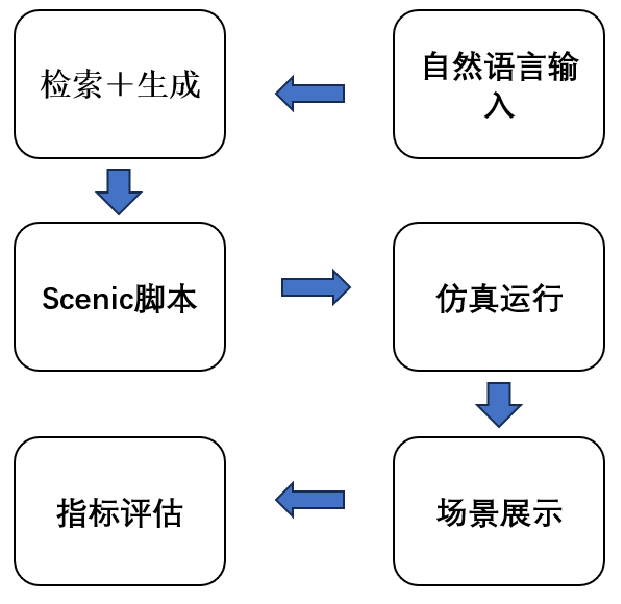
\includegraphics[width=0.9\textwidth]{../images/研究架构图.pdf} 
	\caption{本文的研究框架}
	\label{fig:research_framework}
\end{figure}